\section{Differencing}
\label{sec:pi-diff}

\kl{Differencing}---whether done by the tool (\kl{automatic configuration}) or by the proof engineer (\kl{manual configuration})---identifies 
and proves a type equivalence. But differening further decomposes that equivalence into a form called a \kl{configuration}. 
The configuration is the key to building a proof term transformation that implements transport in a way that is suitable for repair.

Each configuration is a deconstruction of a particular equivalence \Aa $\simeq$ \B.
In particular, it deconstructs the equivalence into things that talk about \Aa, and things that talk about \B.
It does so in a way that hides details
specific to the equivalence, like the order or number of arguments to an \kl{eliminator} or type.

At a high level, the configuration helps the transformation achieve two goals: 

\begin{enumerate}
\item preserve equality up to transport across the equivalence between \Aa and \B (Section~\ref{sec:pi-diff-equiv}), and 
\item produce well-typed terms (Section~\ref{sec:pi-diff-equal}).
\end{enumerate}
To differencing, this configuration is a pair of pairs of terms:

\begin{lstlisting}
  ((DepConstr, DepElim), (Eta, Iota))
\end{lstlisting}
each of which corresponds to one of the two goals:
\lstinline{DepConstr} and \lstinline{DepElim} define how to transform dependent constructors and eliminators, thereby preserving the equivalence, and 
\lstinline{Eta} and \lstinline{Iota} define how to transform $\eta$-expansion and $\iota$-reduction of dependent constructors and eliminators, thereby producing well-typed terms.

The connection between the configuration parts and constructors and eliminators is a bit of an analogy---though one with formal meaning by way of
category theory (Section~\ref{sec:algebra}).
Configurations and equivalences are equally expressive: every configuration induces an equivalence, and every equivalence induces a configuration
(Section~\ref{sec:correct-cic}).
Each search procedure for automatic configuration produces both the configuration and the equivalence that it induces (Section~\ref{sec:proc}).
Manual configuration takes as input the configuration directly.

All terms that I introduce in this section are in \kl{CIC$_{\omega}$} with \kl{primitive eliminators}. % TODO point to other conventions again
Section~\ref{sec:pi-diff-limits} revisits the limitations of differencing from \sysname, 
and Section~\ref{sec:pi-implementation} describes how I scale this from CIC$_{\omega}$ to Coq.

\subsection{Preserving the Equivalence}
\label{sec:pi-diff-equiv}

To preserve the equivalence, the configuration maps terms over \Aa to terms over \B by viewing each
term of type \B as if it were an \Aa.
This way, the transformation in Section~\ref{sec:pi-trans} can replace values of \Aa with values of \B, and
inductive proofs about \Aa with inductive proofs about \B, %, then recursively transform
%subterms 
all without changing the order or number of arguments.

The two configuration parts responsible for this are \lstinline{DepConstr}
and \lstinline{DepElim} (\intro{dependent constructors} and \intro{dependent eliminators}).
These describe how to construct and eliminate \Aa and \B, wrapping the types with a common inductive structure.
The transformation requires the same number of dependent constructors and cases in dependent eliminators for \Aa and \B,
even if \Aa and \B are \kl{inductive types} with different numbers of \kl{constructors}
(\Aa and \B need not even be inductive; see Sections~\ref{sec:art} and~\ref{sec:pi-results}).

\begin{figure*}
\begin{minipage}{0.49\textwidth}
\begin{lstlisting}
(* nil *)
DepConstr(0, Old.list T)
  : Old.list T
:= Constr((@\codediff{0}@), Old.list T).

(* cons *)
DepConstr(1, Old.list T) t l
  : Old.list T
:= Constr ((@\codediff{1}@), Old.list T) t l.

(* induction over lists *)
DepElim(l, P) { p$_{\mathtt{nil}}$, p$_{\mathtt{cons}}$ }
  : P l
:= Elim(l, P) { (@\codediff{p$_{\mathtt{nil}}$}@), (@\codediff{p$_{\mathtt{cons}}$}@) }.
\end{lstlisting}
\end{minipage}
\hfill
\begin{minipage}{0.49\textwidth}
\begin{lstlisting}
(* nil *)
DepConstr(0, New.list T)
  : New.list T
:= Constr((@\codediff{1}@), New.list T).

(* cons *)
DepConstr(1, New.list T) t l
  : New.list T
:= Constr((@\codediff{0}@), New.list T) t l.

(* induction over lists *)
DepElim(l, P) { p$_{\mathtt{nil}}$, p$_{\mathtt{cons}}$ }
  : P l
:= Elim(l, P) { (@\codediff{p$_{\mathtt{cons}}$}@), (@\codediff{p$_{\mathtt{nil}}$}@) }.
\end{lstlisting}
\end{minipage}
\caption{The dependent constructors and eliminators for old (left) and new (right) \lstinline{list}, with the difference in \codediff{orange}.}
\label{fig:listconfig}
\end{figure*}

For the \lstinline{list} change from Section~\ref{sec:overview},
the configuration that \toolnamec discovers uses the dependent constructors
and eliminators in Figure~\ref{fig:listconfig}. The dependent constructors for \lstinline{Old.list}
are the normal constructors with the order unchanged,
while the dependent constructors for \lstinline{New.list} swap constructors
back to the original order.
Similarly, the dependent eliminator for \lstinline{Old.list} is the normal eliminator for \lstinline{Old.list},
while the dependent eliminator for \lstinline{New.list} swaps cases.

As the name hints, these constructors and eliminators can be dependent.
For example, let \B be the type of
vectors of some arbitrary, unspecified length,
packed into a $\Sigma$ type:

\begin{lstlisting}
  $\Sigma$(n : nat).vector T n
\end{lstlisting}
\toolnamec can port proofs across the equivalence between this choice of \B and \lstinline{list T}~\href{https://github.com/uwplse/pumpkin-pi/blob/v2.0.0/plugin/coq/examples/Example.v}{\circled{3}}. % Example.v
The dependent constructors \toolnamec discovers for \B pack the index into an existential, like:

\begin{lstlisting}
  DepConstr(0, B) : B :=
    $\exists$ (Constr(0, nat)) (Constr(0, vector T)).
\end{lstlisting}
and the eliminator it discovers eliminates the projections:

\begin{lstlisting}
  DepElim(b, P) { f$_0$ f$_1$ } : P ($\exists$ ($\pi_l$ b) ($\pi_r$ b)) :=
    Elim($\pi_r$ b, $\lambda$(n : nat)(v : vector T n).P ($\exists$ n v)) {
      f$_0$,
      ($\lambda$(t : T)(n : nat)(v : vector T n).f$_1$ t ($\exists$ n v))
    }.
\end{lstlisting}

In both these examples, the interesting work moves into the configuration:
the configuration for the first swaps constructors and cases,
and the configuration for the second maps constructors and cases over \lstinline{list} to constructors and cases over \lstinline{packed_vect}. %packs constructors and eliminates projections.
That way, the transformation need not add, drop, or reorder arguments---it can truly be generic over type equivalences.
%In essence, all of the difficult work moves into the configuration.
Furthermore, both examples use automatic configuration, so differencing in \toolnamec's \textbf{Configure} component
discovers \lstinline{DepConstr} and \lstinline{DepElim} from just the types \Aa and \B, taking care of even the difficult work.

\subsection{Producing Well-Typed Terms}
\label{sec:pi-diff-equal}

The other configuration parts \lstinline{Eta} and \lstinline{Iota} deal with producing well-typed terms,
in particular by transporting equalities.
Recall that CIC$_{\omega}$ is an \kl{intensional} type theory,
and so distinguishes between \kl{definitional} and \kl{propositional} equality.
When a datatype changes, sometimes, definitional equalities defined over the old version of that type must become propositional.
A naive proof term transformation may fail to generate well-typed terms if it does not account for this.
Otherwise, if the transformation transforms a term $t : T$ to some $t' : T'$, it does not necessarily
transform $T$ to $T'$~\cite{tabareau2019marriage}.

\lstinline{Eta} and \lstinline{Iota} describe how to transport equalities.
More formally, they define \intro{$\eta$}-expansion and \intro{$\iota$}-reduction of \Aa and \B,
which may be propositional rather than definitional,
and so must be explicit in the transformation.
$\eta$-expansion describes how to expand a term to apply a constructor to an eliminator in a way that preserves propositional equality,
and is important for defining dependent eliminators~\cite{nlab:eta-conversion}.
$\iota$-reduction ($\beta$-reduction for inductive types) describes how to reduce an elimination of a constructor~\cite{nlab:beta-reduction}.

The configuration for the change from lists to vectors of some length has propositional \lstinline{Eta} over \B.
It uses $\eta$-expansion for $\Sigma$:

\begin{lstlisting}
  Eta(B) := $\lambda$(b : B).$\exists$ ($\pi_l$ b) ($\pi_r$ b).
\end{lstlisting}
which is propositional and not definitional in Coq.
Thanks to this, we can forego the assumption that our language has primitive projections (definitional $\eta$ for $\Sigma$).

\begin{figure}
\begin{minipage}{0.44\columnwidth}
   \lstinputlisting[firstline=1, lastline=8]{often/nattobin.tex}
\end{minipage}
\hfill
\begin{minipage}{0.54\columnwidth}
   \lstinputlisting[firstline=10, lastline=17]{often/nattobin.tex}
\end{minipage}
\caption{A unary natural number \lstinline{nat} (left) is either zero (\lstinline{0}) or the successor of some other natural number (\lstinline{S}).
A binary natural number \lstinline{N} (right) is either zero (\lstinline{N0}) or a positive binary number (\lstinline{Npos}), where a positive binary number is either 1 (\lstinline{xH}), or the result of shifting left and adding 1 (\lstinline{xI}) or
0 (\lstinline{xO}). While \lstinline{nat} and \lstinline{N} are equivalent, they have different inductive structures.
Consequentially, \kl{definitional} equalities over \lstinline{nat} may become \kl{propositional} over \lstinline{N}.}
\label{fig:nattobin}
\end{figure}

Each \lstinline{Iota}---one per constructor---describes and proves the $\iota$-reduction behavior
of \lstinline{DepElim} on the corresponding case.
This is needed, for example, to port proofs about unary numbers \lstinline{nat} to
proofs about binary numbers \lstinline{N} (Figure~\ref{fig:nattobin}).
While we can define \lstinline{DepConstr} and \lstinline{DepElim} to induce an equivalence
between them~\href{https://github.com/uwplse/pumpkin-pi/blob/v2.0.0/plugin/coq/nonorn.v}{\circled{5}}, % nonorn.v (TODO update links throughout)
we run into trouble reasoning about applications of \lstinline{DepElim},
since proofs about \lstinline{nat} that hold by reflexivity do not necessarily hold by reflexivity over \lstinline{N}. 
For example, in Coq, while \lstinline{S (n + m)  = S n + m} holds by reflexivity over \lstinline{nat},
when we define \lstinline{+} with \lstinline{DepElim} over \lstinline{N},
the corresponding theorem over \lstinline{N} does not hold by reflexivity.

To transform proofs about \lstinline{nat} to proofs about \lstinline{N}, we must transform \kl{definitional} $\iota$-reduction over \lstinline{nat} to 
\kl{propositional} $\iota$-reduction over \lstinline{N}.
For our choice of \lstinline{DepConstr} and \lstinline{DepElim},
$\iota$-reduction is definitional over \lstinline{nat}, since a proof of:

\begin{lstlisting}
  $\forall$ P p$_\texttt{0}$ p$_\texttt{S}$ (n : nat),
    DepElim((@\codediff{DepConstr(1, nat) n}@), P) { p$_\texttt{0}$, p$_\texttt{S}$ } =
    (@\codediff{p$_\texttt{S}$}@) n (DepElim(n, P) { p$_\texttt{0}$, p$_\texttt{S}$ }).
\end{lstlisting}
holds by reflexivity.
\lstinline{Iota} for \lstinline{nat} in the \lstinline{S} case is a rewrite by that proof by reflexivity~\href{https://github.com/uwplse/pumpkin-pi/blob/v2.0.0/plugin/coq/nonorn.v}{\circled{5}},
with type:

\begin{lstlisting}
  $\forall$ P p$_\texttt{0}$ p$_\texttt{S}$ (n : nat) (Q: P (DepConstr(1, nat) n) $\rightarrow$ s),
    Iota(1, nat, Q) :
      Q ((@\codediff{p$_\texttt{S}$}@) n (DepElim(n, P) { p$_\texttt{0}$, p$_\texttt{S}$ })) $\rightarrow$
      Q (DepElim((@\codediff{DepConstr(1, nat) n}@), P) { p$_\texttt{0}$, p$_\texttt{S}$ }).
\end{lstlisting}
In contrast, $\iota$ for \lstinline{N} is propositional, since the 
theorem: %over \lstinline{N}:

\begin{lstlisting}
  $\forall$ P p$_\texttt{0}$ p$_\texttt{S}$ (n : N),
    DepElim((@\codediff{DepConstr(1, N) n}@), P) { p$_\texttt{0}$, p$_\texttt{S}$ } =
    (@\codediff{p$_\texttt{S}$}@) n (DepElim(n, P) { p$_\texttt{0}$, p$_\texttt{S}$ }).
\end{lstlisting}
no longer holds by reflexivity.
\lstinline{Iota} for \lstinline{N} is a rewrite by the propositional equality that proves this theorem~\href{https://github.com/uwplse/pumpkin-pi/blob/v2.0.0/plugin/coq/nonorn.v}{\circled{5}},
with type:

\begin{lstlisting}
  $\forall$ P p$_\texttt{0}$ p$_\texttt{S}$ (n : N) (Q: P (DepConstr(1, N) n) $\rightarrow$ s),
    Iota(1, N, Q) :
      Q ((@\codediff{p$_\texttt{S}$}@) n (DepElim(n, P) { p$_\texttt{0}$, p$_\texttt{S}$ })) $\rightarrow$
      Q (DepElim((@\codediff{DepConstr(1, N) n}@), P) { p$_\texttt{0}$, p$_\texttt{S}$ }).
\end{lstlisting}
By replacing \lstinline{Iota} over \lstinline{nat} with \lstinline{Iota} over \lstinline{N},
the transformation replaces rewrites by reflexivity over \lstinline{nat} to rewrites by propositional equalities over \lstinline{N}.
That way, \lstinline{DepElim} behaves the same over \lstinline{nat} and \lstinline{N}.

Taken together over both \Aa and \B, \lstinline{Iota} describes how the inductive structures of \Aa and \B differ.
The transformation requires that \lstinline{DepElim} over \Aa and over \B have the same structure
as each other, so if \Aa and \B \textit{themselves} have the same 
inductive structure (if they are \textit{ornaments}~\cite{mcbride}),
then if $\iota$ is definitional for \Aa, it will be possible to choose
\lstinline{DepElim} with definitional $\iota$ for \B.
Otherwise, if \Aa and \B (like \lstinline{nat} and \lstinline{N}) have different inductive structures,
then definitional $\iota$ over one would become propositional $\iota$ over the other.

\subsection{Specifying Correct Configurations}
\label{sec:art}

Choosing a configuration necessarily depends in some way on the proof engineer's intentions:
there can be infinitely many equivalences that correspond to a 
change, only some of which are useful (for example~\href{https://github.com/uwplse/pumpkin-pi/blob/v2.0.0/plugin/coq/playground/refine_unit.v}{\circled{7}}, any \Aa is equivalent to \lstinline{unit} refined by \Aa). % refine_unit.v
And there can be many configurations that correspond
to an equivalence, some of which will produce terms that are more useful or efficient than others
(consider \lstinline{DepElim} converting through several intermediate types).

Thankfully, while it is not possible to control for intentions,
it \textit{is} possible to specify what it means for a chosen configuration to be correct.
In particular, the analogy tying the \kl{configuration} to \kl{contructors} and \kl{eliminators} by way of the 
names \lstinline{DepConstr} and \lstinline{DepElim} is not a coincidence.
In fact, it has meaning in terms of what in category theory are known as \intro{initial algebras of endofunctors},
and correctness---that configurations and equivalences are isomorphic---follows by Lambek's 
theorem (Section~\ref{sec:algebra}).
A more syntactic version of this claim can be used to specify and prove correctness of configurations in CIC$_{\omega}$ (Section~\ref{sec:correct-cic}).

\paragraph{Historical Note}
When I met with \kl{Michael Shulman} over coffee a few years ago, he said that a preliminary version of this work ``feels like univalence,'' ``feels like coherence,'' and ``feels like an endofunctor.'' All three were correct! But I didn't understand the connection to endofunctors by way of Lambek's until a few months before writing this thesis.
\kl{Carlo Angiuli} and \kl{Anders M\"{o}rtberg} identified this connection, and \kl{Carlo} explained it to me.
It is quite beautiful!

But it is also quite preliminary. I hope this connection as presented in Section~\ref{sec:algebra} will help 
communicate some of the categorical intuition behind why all of this works, but I will not be surprised if I get some of the details wrong.
Please regard this as a bit speculative, unlike the syntactic presentation in Section~\ref{sec:correct-cic},
which is already published.

\subsubsection{Categorical Intuition for Correctness}
\label{sec:algebra}

\begin{figure}
\begin{center}
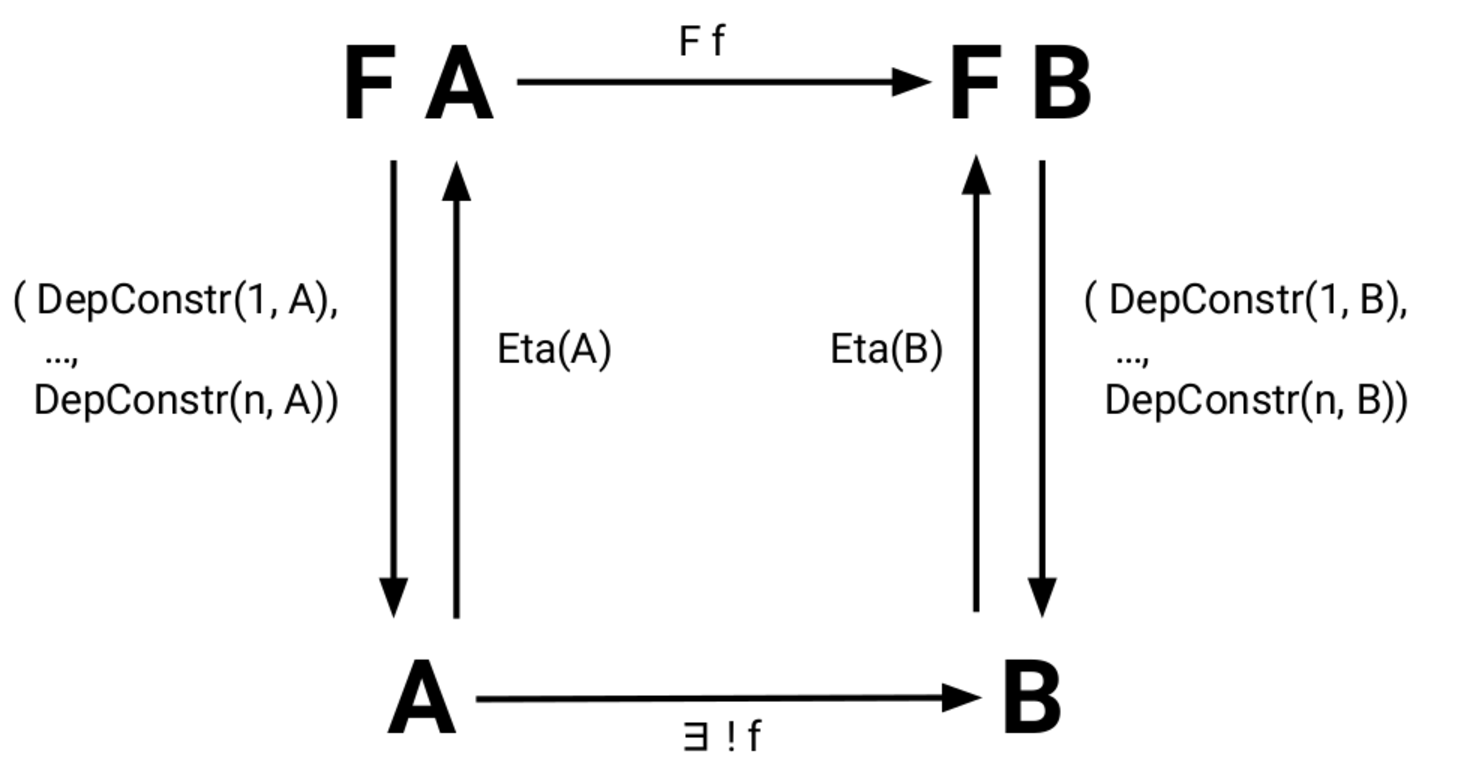
\includegraphics[scale=0.40]{often/Diagram}
\end{center}
\caption{The categorical representation of a configuration for equivalent types \Aa and \B in terms of initial algebras.}
\label{fig:lambek}
\end{figure}

Configurations have meaning in terms of \kl{initial algebras}~\cite{nlab:initial_algebra_of_an_endofunctor},
which in \kl{homotopy type theory} represent inductive types~\cite{univalent2013homotopy}.
This is why the configuration is most natural when the types \Aa and \B are inductive.
But the configuration is in fact more general than that---it can support any two equivalent types \Aa and \B (by Lambek's theorem).

Figure~\ref{fig:lambek} shows this for an arbitrary configuration for an equivalence between \Aa and \B.
Here, $F\ A$ is the shape of \Aa.
\lstinline{DepConstr} maps from $F\ A$ to \Aa, and \lstinline{Eta} maps from \Aa back to $F\ A$.
\lstinline{DepElim} (not pictured explicitly) is the arrow corresponding to \lstinline{DepConstr} defined over the analogous diagram
lifted to $A \rightarrow$ $s$ for some sort $s$ (also not pictured explicitly);
by uniqueness of \lstinline{f}, any \lstinline{f} must pass through a function 
isomorphic to \lstinline{DepElim}.
\lstinline{Iota} (also not pictured explicitly) is used in the proof that the diagram commutes.
The configuration parts for \B are similar.

For example, fixing \Aa as \lstinline{nat}, $F\ A$ is \lstinline{1 + nat}:
the sum of the unit type and \lstinline{nat}.
Going from $F\ A \rightarrow A$, the left injection maps to the \lstinline{O} constructor, and the right injection maps to the \lstinline{S} constructor.
The inverse is essentially\footnote{Some differences in the type theory make this not quite perfect.} the identity function.
Any $f$ must pass through the eliminator for \lstinline{nat}, which would show up explicitly in place of the constructors
in the diagram lifted to \lstinline{nat} $\rightarrow$ $s$.
The diagram commutes trivially, since the \lstinline{S} case of the eliminator reduces.

This diagram gives intuition for how the configuration splits up an arbitrary equivalence between \Aa and \B into
parts that talk about \Aa and \B separately. All the transformation in Chapter~\ref{sec:pi-trans} does is follow the arrows
in the diagram to get from \Aa directly to \B.
But in order to do that, it needs to handle the nuances of \kl{definitional equality} and dependent types in \kl{CIC${_\omega}$}---for example,
by explicitly representing and porting the proof that the diagram commutes.
The syntactic presentation in the next section handles those nuances.

\subsubsection{Correctness in CIC$_{\omega}$}
\label{sec:correct-cic}

\begin{figure*}
\begin{lstlisting}
(* -------------------- Equivalence -------------------- *)

section: $\forall$ (a : A) . g (f a) = a.
retraction: $\forall$ (b : B), f (g b) = b.

constr_ok:
  $\forall$ $j$ $\vec{x_A}$ $\vec{x_B}$,
    $\vec{x_A}$ $\equiv_{A \simeq B}$ $\vec{x_B}$ $\rightarrow$
    DepConstr($j$, A) $\vec{x_A}$ $\equiv_{A \simeq B}$ DepConstr(j, B) $\vec{x_B}$.

elim_ok:
  $\forall$ a b P$_A$ P$_B$ $\vec{f_A}$ $\vec{f_B}$,
    a $\equiv_{A \simeq B}$ b $\rightarrow$
    P$_A$ $\equiv_{(A \rightarrow s) \simeq (B \rightarrow s)}$ P$_B$ $\rightarrow$
    ($\forall$ $j$, $\vec{f_A}$[j] $\equiv_{\xi (A, P_A, j) \simeq \xi (B, P_B, j)}$ $\vec{f_B}$[j]) $\rightarrow$
    DepElim(a, P$_A$) $\vec{f_A}$ $\equiv_{(P a) \simeq (P b)}$ DepElim(b, P$_B$) $\vec{f_A}$.


(* ---------------------- Equality ---------------------- *)

elim_eta(A): $\forall$ a P $\vec{f}$, DepElim(a, P) $\vec{f}$ : P (Eta(A) a).
eta_ok(A): $\forall$ (a : A), Eta(A) a = a.

iota_ok(A):
  $\forall$ $j$ P $\vec{f}$ $\vec{x}$ (Q: P(Eta(A) (DepConstr($j$, A) $\vec{x}$)) $\rightarrow$ s),
    Iota(A, j, Q) : 
      Q (DepElim(DepConstr(j, A) $\vec{x}$, P) $\vec{f}$) $\rightarrow$ 
      Q (rew $\leftarrow$ eta_ok(A) (DepConstr(j, A) $\vec{x}$) in 
        ($\vec{f}$[j]$\ldots$(DepElim(IH$_0$, P) $\vec{f}$)$\ldots$(DepElim(IH$_n$, P) $\vec{f}$)$\ldots$)).
\end{lstlisting}
\caption{Correctness criteria for a configuration to ensure that the transformation
preserves equivalence (top) coherently with equality (bottom, shown for \Aa; \B is similar). \lstinline{f} and \lstinline{g} are defined in text. $s$, $\vec{f}$, $\vec{x}$, and $\vec{\mathtt{IH}}$ represent
sorts, \kl{eliminator} cases, \kl{constructor} arguments, and \kl{inductive hypotheses}. $\xi$ $(A,$ $P,$ $j)$ is the type 
of \lstinline{DepElim(A, P)} at \lstinline{DepConstr(j, A)} (similarly for \B).
\lstinline{rew} is shorthand for applying the equality eliminator.} %, respectively.}
\label{fig:spec}
\end{figure*}

The categorical definition may help with some of the intuition, but it does not help with validating correct configurations inside of the type theory.
Fortunately, in CIC$_{\omega}$, it is also possible to specify 
what it means for a chosen configuration to be correct:
Fix a configuration. Let \lstinline{f} be the function that uses \lstinline{DepElim} to eliminate \Aa and \lstinline{DepConstr} to construct \B,
and let \lstinline{g} be similar.
Figure~\ref{fig:spec} specifies the correctness criteria for the configuration.
These criteria relate \lstinline{DepConstr}, \lstinline{DepElim}, \lstinline{Eta}, and \lstinline{Iota}
in a way that preserves equivalence coherently with equality.

\paragraph{Equivalence}
To preserve the equivalence (Figure~\ref{fig:spec}, top), \lstinline{DepConstr} and \lstinline{DepElim} must form an equivalence
(\lstinline{section} and \lstinline{retraction} must hold for \lstinline{f} and \lstinline{g}).
\lstinline{DepConstr} over \Aa and \B must be equal up to transport across that equivalence (\lstinline{constr_ok}), 
and similarly for \lstinline{DepElim} (\lstinline{elim_ok}).
Intuitively, \lstinline{constr_ok} and \lstinline{elim_ok} guarantee that the transformation
correctly transports dependent constructors and dependent eliminators,
as doing so will preserve equality up to transport for those subterms.
This makes it possible for the transformation
to avoid applying \lstinline{f} and \lstinline{g}, instead porting terms from \Aa directly to \B.

\paragraph{Equality}
To ensure coherence with equality (Figure~\ref{fig:spec}, bottom),
\lstinline{Eta} and \lstinline{Iota} must prove $\eta$ and $\iota$.
That is, \lstinline{Eta} must have the same definitional behavior as the dependent eliminator (\lstinline{elim_eta}),
and must behave like identity (\lstinline{eta_ok}).
Each \lstinline{Iota} must prove and rewrite along the simplification (\textit{refolding}~\cite{boutillier:tel-01054723}) behavior that corresponds to a case of the dependent eliminator (\lstinline{iota_ok}).
This makes it possible for the transformation to
avoid applying \lstinline{section} and \lstinline{retraction}.

\paragraph{Correctness}
With these correctness criteria for a configuration, we get the completeness result (proven in Coq~\href{https://github.com/uwplse/pumpkin-pi/blob/v2.0.0/plugin/coq/playground/arbitrary.v}{\circled{8}}) that every equivalence induces a configuration. % arbitrary.v
We also obtain an algorithm for the soundness result that every configuration induces an equivalence.
Both of these are what we would expect from Lambek's theorem, which states that the initial algebra and the equivalence are isomorphic to one another.

The algorithm to prove \lstinline{section} is as follows (\lstinline{retraction} is similar):
replace \lstinline{a} with \lstinline{Eta(A) a} by \lstinline{eta_ok(A)}.
Then, induct using \lstinline{DepElim} over \Aa.
For each case $j$, the proof obligation is to show that \lstinline{g (f a)} is equal to \lstinline{a},
where \lstinline{a} is \lstinline{DepConstr(A, j)} applied to the non-inductive arguments (by \lstinline{elim_eta(A)}).
Expand the right-hand side using \lstinline{Iota(A, j)}, then expand it again using \lstinline{Iota(B, j)}
(destructing over each \lstinline{eta_ok} to apply the corresponding \lstinline{Iota}).
The result follows by definition of \lstinline{g} and \lstinline{f}, and by reflexivity.

\paragraph{Equivalences from Configurations}
The algorithm above is essentially what differencing uses for each search procedure to generate functions \lstinline{f} and \lstinline{g} for the automatic configurations~\href{https://github.com/uwplse/pumpkin-pi/blob/v2.0.0/plugin/src/automation/search/search.ml}{\circled{9}}, % search.ml
and also generate proofs \lstinline{section} and \lstinline{retraction} that these functions form an equivalence~\href{https://github.com/uwplse/pumpkin-pi/blob/v2.0.0/plugin/src/automation/search/equivalence.ml}{\circled{10}}. % equivalence.ml
To minimize dependencies, \toolnamec does not produce proofs of \lstinline{constr_ok} and \lstinline{elim_ok} directly,
as stating these theorems cleanly would require either a special framework~\cite{tabareau2017equivalences}
or a univalent type theory~\cite{univalent2013homotopy}.
If the proof engineer wishes, it is possible to prove these in individual cases~\href{https://github.com/uwplse/pumpkin-pi/blob/v2.0.0/plugin/coq/playground/arbitrary.v}{\circled{8}}, % arbitray.v
but this is not necessary in order to use \toolnamec. %---they simply need to hold.
% TODO not quite true

\subsection{Search Procedures}
\label{sec:proc}

\toolnamec implements four search procedures for \kl{automatic configuration}~\href{https://github.com/uwplse/pumpkin-pi/blob/v2.0.0/plugin/src/automation/lift/liftconfig.ml}{\circled{6}}:

\begin{enumerate}
\item algebraic ornaments,
\item unpacking $\Sigma$ types,
\item swapping constructors, and
\item moving between nested pairs and records.
\end{enumerate}
As a courtesy to the reader, in this section, I detail just the first search procedure as an example.
In Section~\ref{sec:pi-implementation}, I will briefly describe the other search procedures,
as well as what is needed to extend \toolnamec with new search procedures.
I will also explain how the search procedures are implemented.

% DEVOID 3.1 adjusted

The first search procedure discovers equivalences that correspond to \intro{algebraic ornaments}.
An algebraic ornament relates an \kl{inductive type} to an indexed version of that type,
where the new index is fully determined by a unique fold over \Aa (I call this fold the \intro{indexer}). 
For example, \lstinline{vector} is exactly \lstinline{list} with a new index of type \lstinline{nat},
where the new index is fully determined by the \lstinline{length} function (recall Figure~\ref{fig:listtovect} on page~\pageref{fig:listtovect}).
The equivalence that we already saw in Section~\ref{sec:pi-scope} follows from this:

\begin{lstlisting}
  $\Sigma$(l : list T).length l = n $\simeq$ vector T n
\end{lstlisting}
Alternatively, we can say that a list is equivalent to a vector of \textit{some} length:

\begin{lstlisting}
  list T $\simeq$ $\Sigma$(n : nat).vector T n
\end{lstlisting}
As usual, this equivalence is made up of two functions \lstinline{f} and \lstinline{g}, along with proofs \lstinline{section} and \lstinline{retraction}.
In addition, for algebraic ornaments, there is a proof of this theorem:

\begin{lstlisting}
  $\forall$ (l : list T), length l = $\pi_{l}$ (f l)
\end{lstlisting}
which states that the \lstinline{length} function is \intro{coherent} with this equivalence.

In Section~\ref{sec:pi-results}, I will show you a case study of porting functions and proofs from lists to length-indexed vectors.
Nominally this works by porting the functions and proofs along the equivalence from Section~\ref{sec:pi-scope},
but in practice this works by chaining two different automatic configurations with some human input.
The first configuration uses a search procedure that discovers the equivalence between lists and vectors of some length above,
as well as the proof of coherence.
The second configuration uses a search procedure that discovers how to unpack vectors of some length to vectors of a \textit{particular} length.

The first configuration nicely demonstrates how differencing works, so let us look at this in detail.
Assume the existence of inductive types \Aa and \AI, related by an algebraic ornament with the index of type \I.
In the scope of this thesis, further assume that \Aa and \I are not indexed types.\footnote{The original paper that this is from lets all of \Aa,
\AI, and \I be \textit{indexed} inductive types, with the new index of type \I appearing anywhere within the list of indices of \AI;
the implementation makes the same decision.
I felt that this was very important to show in detail when I wrote that paper, since indices are often omitted,
even though handling them is one of the trickiest parts of implementing an algorithm like this.
In this thesis, however, I decided to simplify the presentation and assume the types are not indexed,
and so the new index is the only index of \AI.
I do recommend checking out the original paper if you would really like to implement something like this over indexed types---it is formalized
those who are \textit{sufficiently fanatical}.}
Then there is a type equivalence:

\begin{lstlisting}
  $A\ \simeq\ \Sigma (i : I).A_I\ i$
\end{lstlisting}
In addition, there is an \kl{indexer}, which is a unique fold:

\begin{lstlisting}
  indexer : $A\ \rightarrow\ I$.
\end{lstlisting}
that projects the lifted index:

\begin{lstlisting}
  coherence : $\forall (a : A),\ $indexer$\ a = \pi_{l}\ ($f$\ a)$.
\end{lstlisting}
Following existing work, I call this equivalence the \intro{ornamental promotion isomorphism}~\cite{ko2016programming}; 
when it holds and a \kl{coherent} indexer exists, I say that \AI is an \kl{algebraic ornament} of \Aa.

In their original form, ornaments are a programming mechanism: given a type \Aa, an ornament determines
some new type \AI. Differencing inverts this process for algebraic ornaments: given types \Aa\ and \AI, 
it searches for the configuration that induces the ornamental promotion isomorphism between them.
This is possible for algebraic ornaments precisely because the indexer is extensionally unique.
For example, all possible indexers for \lstinline{list} and \lstinline{vector} must compute
the length of a list; if we were to try doubling the length instead, we would not be able to satisfy the equivalence.

% DEVOID 4.1 mostly unchanged

\paragraph{Common Definitions}
The algorithm assumes a function \lstinline{new} that determines whether a hypothesis in a case of the eliminator type of \AI\ is new.
Figure~\ref{fig:common} contains other common definitions, the names for which are reserved:
Input type \Aa\ expands to an inductive type with constructors
\smallmath{$\{\mathrm{C}_{A_1}, \ldots, \mathrm{C}_{A_n}\}$}.
\smallmath{$\mathrm{P}_A$} denotes the type of the motive of the eliminator of \Aa,
and each \smallmath{$\mathrm{E}_{A_j}$} denotes the type of the eliminator for the $j$th constructor of \Aa.
Analogous names are also reserved for input type \AI.
The type \B is \AI at some index of type \I.

\begin{figure}
\begin{lstlisting}
$A$ := $\mathrm{Ind} (\mathit{Ty}_A : \mathrm{s}_A)\{\mathrm{C}_{A_1}, \ldots, \mathrm{C}_{A_n}\}$
$A_I$ := $\mathrm{Ind} (\mathit{Ty}_{A_I} : (\Pi (i : I). \mathrm{s}_{A_I}))\{\mathrm{C}_{A_{I_1}}, \ldots, \mathrm{C}_{A_{I_n}}\}$
$B$ := $\Sigma (i : I) . A_I i$

$\mathrm{P}_A$ := $\Pi (a : A) . \mathrm{s}_A$
$\mathrm{P}_{A_I}$ := $\Pi (i : I) (a_i : A_I\ i) . \mathrm{s}_{A_I}$

$\forall 1 \le j \le n,$
  $\mathrm{E}_{A_j}\ (p_A : \mathrm{P}_A)$ := $\xi(A,\ p_A,\ j)$
  $\mathrm{E}_{B_j}\ (p_{A_I} : \mathrm{P}_{A_I})$ := $\xi(A_I,\ p_{A_I},\ j)$
\end{lstlisting}
\caption{Common definitions. Here, $\xi$ $(A,$ $p_A$, $j)$ is the type 
of \lstinline{Elim(A, p}$_A$\lstinline{)} at \lstinline{Constr(j, A)} (similarly for $A_I$).}
\label{fig:common}
\end{figure}

For historical reasons, differencing generates the equivalence first, then derives the configuration, rather than the other way around. % TODO fix if time
It builds on three intermediate steps: one to generate each of \lstinline{indexer},
\lstinline{f}, and \lstinline{g}.
It then uses that to build the configuration.
Figure~\ref{fig:searchindexer} shows the algorithm for generating \lstinline{indexer}.
The algorithms for generating \lstinline{f} and \lstinline{g} are similar;
Figure~\ref{fig:searchpromote} shows only the derivations for generating \lstinline{f}
that are different from those for generating \lstinline{indexer}, and 
the derivations for generating \lstinline{g} are omitted.

\subsubsection{Differencing for the Indexer}

Then differencing algorithm generates the \lstinline{indexer} by traversing the types of the eliminators for \Aa\ and \AI\ in parallel using the algorithm from Figure~\ref{fig:searchindexer},
which consists of three judgments: one to generate the \kl{motive}, one to generate each case,
and one to compose the motive and cases.

\begin{figure}
\begin{mathpar}
%\begin{minipage}{0.45\textwidth}
\mprset{flushleft} 
\small
\hfill\fbox{$\Gamma$ $\vdash$ $(T_A,\ T_{A_I}) \Downarrow_{i_{m}} t$ }\vspace{-0.55cm}\\

\inferrule[Index-Motive] 
  { \\ }
  { \Gamma \vdash (A, A_I) \Downarrow_{i_{m}} \lambda (a : A) . I }\\

\hfill\phantom{woooooooooooooooooooooooooooooooooooooooooooooooo}\fbox{$\Gamma$ $\vdash$ $(T_A,\ T_{A_I}) \Downarrow_{i_{c}} t$ }\vspace{-0.4cm}\\

\inferrule[Index-Conclusion]
  { \\ }
  { \Gamma \vdash (p_A\ a,\ p_{A_I}\ i\ a_i) \Downarrow_{i_{c}} i } 

\inferrule[Index-Hypothesis] % new hypothesis for index
  { \mathrm{new}\ n_{A_I}\ b_{A_I} \\\\ \Gamma,\ n_{A_I} : t_{A_I} \vdash (\Pi (n_A : t_A) . b_A,\ b_{A_I}) \Downarrow_{i_{c}} t }
  {  \Gamma \vdash (\Pi (n_A : t_A) . b_A,\ \Pi (n_{A_I} : t_{A_I}) . b_{A_I}) \Downarrow_{i_{c}} t}

\inferrule[Index-IH] % inductive hypothesis
  { \Gamma \vdash (A, A_I) \Downarrow_{i_{m}} p \\
    \Gamma,\ n_A : p\ a \vdash (b_A,\ b_{A_I} [n_A / i]) \Downarrow_{i_{c}} t }
  { \Gamma \vdash (\Pi (n_A : p_A\ a) . b_A,\ \Pi (n_{A_I} : p_{A_I}\ i\ b) . b_{A_I}) \Downarrow_{i_{c}} \lambda (n_A : p\ a) . t }

\inferrule[Index-Prod] % otherwise, unchanged (when we get rid of the gross fall-through thing, needs not new, and needs to check t_A and t_B not IHs)
  { \Gamma,\ n_A : t_A \vdash (b_A,\ b_{A_I} [n_A / n_{A_I}]) \Downarrow_{i_{c}} t }
  { \Gamma \vdash (\Pi (n_A : t_A) . b_A,\ \Pi (n_{A_I} : t_{A_I}) . b_{A_I}) \Downarrow_{i_{c}} \lambda (n_A : t_A) . t }\\

\hfill\phantom{woooooooooooooooooooooooooooooooooooooooooooooooo}\fbox{$\Gamma$ $\vdash$ $(T_A,\ T_{A_I}) \Downarrow_{i} t$ }\vspace{-0.5cm}\\

\inferrule[Index-Ind] 
  { \Gamma \vdash (A,\ A_I) \Downarrow_{i_{m}} p \\
    \Gamma,\ p_A : \mathrm{P}_A,\ p_{A_I} : \mathrm{P}_{A_I} \vdash \{ (\mathrm{E}_{A_1}\ p_A,\ \mathrm{E}_{A_{I_1}}\ p_{A_I}),\ldots,(\mathrm{E}_{A_n}\ p_A,\ \mathrm{E}_{A_{I_n}}\ p_{A_I}) \} \Downarrow_{i_{c}} \vec{f} } 
  { \Gamma \vdash (A,\ A_I) \Downarrow_{i} \lambda (a : A) . \mathrm{Elim}(a, p) \vec{f}}
\end{mathpar}
\caption{Differencing for the indexer function.}
\label{fig:searchindexer}
\end{figure}

\paragraph{Generating the Motive}
The \smallmath{$(T_A,\ T_{A_I}) \Downarrow_{i_{m}} t$} judgment consists of only the derivation \textsc{Index-Motive},
which computes the indexer motive from the types \Aa\ and \AI\ (expanded in Figure~\ref{fig:common}).
It does this by constructing a function from \Aa to \I.
Consider \lstinline{list} and \lstinline{vector}:

\begin{lstlisting}
  list T := Ind (Ty$_A$ : $s$) {$\ldots$}
  vector T := Ind (Ty$_B$ : $\Pi$(@\codediff{(n : nat)}@).$s$) {$\ldots$}
\end{lstlisting}
For these types, \textsc{Index-Motive} computes the motive:

\begin{lstlisting}
  $\Gamma$ $\vdash$ (list T, vector T) $\Downarrow_{i_{m}}$ $\lambda$ (l : list T) . nat
\end{lstlisting}
which is the motive for the length function.

\paragraph{Generating Each Case}
The \smallmath{$\Gamma$ $\vdash$ $(T_A,\ T_{A_I}) \Downarrow_{i_{c}} t$} judgment generates each case of the indexer
by traversing in parallel the corresponding cases of the eliminator types for \Aa\ and \AI.
It consists of four derivations:
\textsc{Index-Conclusion} handles base cases and conclusions of inductive cases,
while \textsc{Index-Hypothesis}, \textsc{Index-IH}, and \textsc{Index-Prod} recurse into
products.

\textsc{Index-Hypothesis} handles each new hypothesis that corresponds to a new index in an \kl{inductive hypothesis}
of an inductive case of the eliminator type for \AI. It adds the new index to the environment, then recurses into the body of only the
type for which the index already exists. For example, in the inductive case of \lstinline{list} and \lstinline{vector}:
\lstinline{new} determines that \lstinline{n} is the new hypothesis.
\textsc{Index-Hypothesis} then recurses into the body of only the \lstinline{vector} case:

\begin{lstlisting}
  $\Pi$ (l : list T) (IH$_l$ : p$_A$ l), p$_A$ (cons t$_l$ l)
  $\Pi$ (v : vector T n) (IH$_v$ : p$_{A_I}$ (@\codediff{n}@) v), p$_{A_I}$ (@\codediff{(S n)}@) (cons (@\codediff{n}@) t$_l$ l)
\end{lstlisting}
\textsc{Index-Prod} is next. It recurses into product types when the hypothesis is neither a new index nor an inductive hypothesis. Here, it runs twice, recursing into the body and substituting names %appropriately
until it hits the inductive hypothesis for both types:

\begin{lstlisting}
  $\Pi$ (IH$_l$ : p$_A$ l), p$_A$ (cons t$_l$ l)
  $\Pi$ (IH$_v$ : p$_{A_I}$ (@\codediff{n}@) l), p$_{A_I}$ (@\codediff{(S n)}@) (cons (@\codediff{n}@) t$_l$ l)
\end{lstlisting}
\textsc{Index-IH} then takes over. It substitutes the new motive in the inductive hypothesis, then recurses into both bodies, 
substituting the new inductive hypothesis for the index in the eliminator type for \AI.
Here, it substitutes the new motive
for \smallmath{$\mathrm{p}_A$} in the type of \lstinline{IH$_l$}, extends the environment with \lstinline{IH$_l$}, then 
substitutes \lstinline{IH$_l$} for \lstinline{n}, so that it recurses on these types:

\begin{lstlisting}
  p$_A$ (cons t$_l$ l)
  p$_{A_I}$ (@\codediff{(S IH$_l$)}@) (cons (@\codediff{IH$_l$}@) t$_l$ l)
\end{lstlisting}
Finally, \textsc{Index-Conclusion} computes the conclusion by taking the new index of the application of the motive \smallmath{$p_{A_I}$},
here \lstinline{S IH$_l$}.
In total, this produces a function:

\begin{lstlisting}
  $\Gamma$ $\vdash$ ($\Pi$$\hspace{-0.08cm}$ (l$\hspace{-0.08cm}$ :$\hspace{-0.08cm}$ list$\hspace{-0.08cm}$ T)$\hspace{-0.08cm}$ (IH$_l$$\hspace{-0.08cm}$ :$\hspace{-0.08cm}$ p$_A$$\hspace{-0.08cm}$ l),$\hspace{-0.08cm}$ p$_A$$\hspace{-0.08cm}$ (cons$\hspace{-0.08cm}$ t$_l$$\hspace{-0.08cm}$ l),$\hspace{-0.08cm}$
        $\Pi$$\hspace{-0.08cm}$ (v$\hspace{-0.08cm}$ :$\hspace{-0.08cm}$ vector$\hspace{-0.08cm}$ T$\hspace{-0.08cm}$ n)$\hspace{-0.08cm}$ (IH$_v$$\hspace{-0.08cm}$ :$\hspace{-0.08cm}$ p$_{A_I}$$\hspace{-0.08cm}$ n$\hspace{-0.08cm}$ v),$\hspace{-0.08cm}$ p$_{A_I}$$\hspace{-0.08cm}$ (S$\hspace{-0.08cm}$ n)$\hspace{-0.08cm}$ (cons$\hspace{-0.08cm}$ n$\hspace{-0.08cm}$ t$_l$$\hspace{-0.08cm}$ l))
    $\Downarrow_{i_{c}}$ $\lambda$$\hspace{-0.08cm}$ (t$_l$$\hspace{-0.08cm}$ :$\hspace{-0.08cm}$ T)$\hspace{-0.08cm}$ (l$\hspace{-0.08cm}$ :$\hspace{-0.08cm}$ list$\hspace{-0.08cm}$ T)$\hspace{-0.08cm}$ (IH$_l$$\hspace{-0.08cm}$ :$\hspace{-0.08cm}$ ($\lambda$$\hspace{-0.08cm}$ (l$\hspace{-0.08cm}$ :$\hspace{-0.08cm}$ list$\hspace{-0.08cm}$ T)$\hspace{-0.08cm}$ .$\hspace{-0.08cm}$ nat)$\hspace{-0.08cm}$ l)$\hspace{-0.08cm}$ .$\hspace{-0.08cm}$ S$\hspace{-0.08cm}$ IH$_l$
\end{lstlisting}
that computes the length of \lstinline{cons t l}.

\paragraph{Composing the Result}
The \smallmath{$\Gamma$ $\vdash$ $(T_A,\ T_{A_I}) \Downarrow_{i} t$} judgment consists of only \textsc{Index-Ind}, which 
identifies the motive and each case using the other two judgments, then composes the result. In the case of \lstinline{list} and \lstinline{vector},
this produces a function:
\begin{lstlisting}
  $\Gamma$ $\vdash$ (list$\hspace{-0.08cm}$ T,$\hspace{-0.08cm}$ vector$\hspace{-0.08cm}$ T)$\hspace{-0.08cm}$
    $\Downarrow_{i}$ $\lambda$$\hspace{-0.08cm}$ (l$\hspace{-0.08cm}$ :$\hspace{-0.08cm}$ list$\hspace{-0.08cm}$ T).
         Elim(l,$\hspace{-0.08cm}$ $\lambda$$\hspace{-0.08cm}$ (l$\hspace{-0.08cm}$ :$\hspace{-0.08cm}$ list$\hspace{-0.08cm}$ T)$\hspace{-0.08cm}$ .$\hspace{-0.08cm}$ nat)$\hspace{-0.08cm}$ {
           O, 
           $\lambda$$\hspace{-0.10cm}$ (t$_l$$\hspace{-0.08cm}$ :$\hspace{-0.08cm}$ T)$\hspace{-0.08cm}$ (l$\hspace{-0.08cm}$ :$\hspace{-0.08cm}$ list$\hspace{-0.08cm}$ T)$\hspace{-0.08cm}$ (IH$_l$$\hspace{-0.08cm}$ :$\hspace{-0.08cm}$ ($\lambda$$\hspace{-0.10cm}$ (l$\hspace{-0.08cm}$ :$\hspace{-0.08cm}$ list$\hspace{-0.08cm}$ T)$\hspace{-0.10cm}$ .$\hspace{-0.08cm}$ nat)$\hspace{-0.08cm}$ l)$\hspace{-0.10cm}$ .$\hspace{-0.08cm}$ S$\hspace{-0.08cm}$ IH$_l$
         }
\end{lstlisting}
that computes the length of a list.

\subsubsection{Differencing for the Configuration}

As mentioned earlier, for historical reasons, differencing in \toolnamec discovers the equivalence parts \lstinline{f} and \lstinline{g} first, then uses
those functions to discover the configuration, rather than the other way around.
It also proves that these functions form an equivalence, and that the indexer is coherent with the equivalence.

\paragraph{Discovering the Equivalence Parts}
Figure~\ref{fig:searchpromote} shows the interesting derivations for the judgment \smallmath{$(T_A,\ T_B) \Downarrow_f t$}
that searches for \lstinline{f}:
\textsc{F-Motive} identifies the motive 
as \B\ with a new index (which it computes using \lstinline{indexer}, denoted by metavariable \smallmath{$\pi$}).
When \textsc{F-IH} recurses, it substitutes the inductive hypothesis for the term rather than
for its index, and it substitutes the new index (which it also computes using \lstinline{indexer}) inside of that term.
\textsc{F-Conclusion} returns the entire term, rather than its index.
Finally, \textsc{F-Ind} not only recurses into each case, but also packs the result into an existential.

%The differencing algorithm is in Figure~\ref{searchconfig}.
%It builds on five intermediate steps: one to generate \lstinline{indexer} (Figure~\ref{fig:searchindexer}),
%and one to generate each of the configuration parts (Figures~\ref{searchconstr}, \ref{searchelim}, \ref{searcheta}, and~\ref{searchiota}).

\begin{figure}
\begin{mathpar}
\mprset{flushleft}  
\small
\hfill\phantom{woooooooooooooooooooooooooooooooooooooooooooooooo}\fbox{$\Gamma$ $\vdash$ $(T_A,\ T_B) \Downarrow_{f_{m}} t$ }\vspace{-0.55cm}\\

\inferrule[F-Motive]
  { \Gamma \vdash (A,\ A_I) \Downarrow_{i} \pi }
  { \Gamma \vdash (A,\ A_I) \Downarrow_{f_{m}} \lambda (a : A) . A_I\ (\pi\ \vec{i_a}\ a) }\\

\hfill\phantom{woooooooooooooooooooooooooooooooooooooooooooooooo}\fbox{$\Gamma$ $\vdash$ $(T_A,\ T_B) \Downarrow_{f_{c}} t$ }\vspace{-0.4cm}\\

\inferrule[F-Conclusion]
  { \\ }
  { \Gamma \vdash (p_A\ a,\ p_{A_I}\ i\ a_i) \Downarrow_{f_{c}} a_i }

\inferrule[F-IH] % inductive hypothesis
  { \Gamma \vdash (A,\ A_I) \Downarrow_{i} \pi \\
    \Gamma \vdash (A,\ A_I) \Downarrow_{f_{m}} p \\\\
    \Gamma,\ n_A : p\ a \vdash (b_A,\ b_{A_I} [n_A / a_i] [\pi\ a / i]) \Downarrow_{p_{c}} t }
  { \Gamma \vdash (\Pi (n_A : p_A\ a) . b_A,\ \Pi (n_{A_I} : p_{A_I}\ i\ a_i) . b_{A_I}) \\\\
    \phantom{\Gamma} \Downarrow_{p_{c}}  \lambda (n_A : p\ a) . t }

\hfill\phantom{woooooooooooooooooooooooooooooooooooooooooooooooo}\fbox{$\Gamma$ $\vdash$ $(T_A,\ T_B) \Downarrow_{f} t$ }\vspace{-0.5cm}\\

\inferrule[F-Ind] 
  { \Gamma \vdash (A,\ A_I) \Downarrow_{i} \pi \\
    \Gamma \vdash (A,\ A_I) \Downarrow_{f_{m}} p \\\\
    \Gamma,\ p_A : \mathrm{P}_A,\ p_{A_I} : \mathrm{P}_{A_I} \vdash \{ (\mathrm{E}_{A_1}\ p_A,\ \mathrm{E}_{A_{I_1}}\ p_{A_I}),\ldots,(\mathrm{E}_{A_n}\ p_A,\ \mathrm{E}_{A_{I_n}}\ p_{A_I}) \} \Downarrow_{p_{c}} \vec{f} } 
  { \Gamma \vdash (A,\ A_I) \Downarrow_{p} \lambda (a : A) . \exists\ (\pi\ a)\ (\mathrm{Elim}(a, p) \vec{f})}
\end{mathpar}
\caption{Differencing for \lstinline{f}.}
\label{fig:searchpromote}
\end{figure} % TODO check this

The omitted derivations to difference for \lstinline{g} are similar,
except that the domain and range are switched. Consequentially, \lstinline{indexer} is never needed;
\textsc{G-Motive} removes the index rather than inserting it, and \textsc{G-IH} no longer substitutes the index.
Additionally, \textsc{G-Hypothesis} adds the hypothesis for the new index
rather than skipping it, and \textsc{G-Ind} eliminates over the projection rather than packing the result. %of applying the eliminator.

\paragraph{Deriving the Configuration}
\textsc{DepConstr} and \textsc{DepElim} over \Aa are just the standard constructors and eliminators for \Aa.
To derive \textsc{DepConstr} over \B, differencing takes each constructor of \Aa,
applies \lstinline{f} to the conclusion of that constructor, and normalizes the result. % TODO refolding
It then ports the hypotheses of the resulting constructor to use \B in place of \Aa, and drops the remaining applications of \lstinline{f}
and the indexer in the body, replacing them instead with the projections $\pi_r$ and $\pi_l$, respectively.

For example, earlier, letting \Aa be lists, \AI be vectors, and \B be vectors of some length,
I noted that the empty constructor of \B packs the constructor of \AI into an existential:

\begin{lstlisting}
  DepConstr(0, $\Sigma$(n : nat).vector T n) : $\Sigma$(n : nat).vector T n :=
    $\exists$ (Constr(0, nat)) (Constr(0, vector T)).(@\vspace{-0.05cm}@)
\end{lstlisting}
This is the same as applying the function \lstinline{f} that \toolnamec derives to the empty list constructor 
\lstinline{Constr(0, list T)}, and then normalizing the result.
On the other hand, the \lstinline{cons} constructor over \B not just packs the result into an existential,
but also takes \B itself as an argument rather than \Aa:

\begin{lstlisting}
  DepConstr(1, $\Sigma$(n : nat).vector T n) : T $\rightarrow$ $\Sigma$(n : nat).vector T n $\rightarrow$ $\Sigma$(n : nat).vector T n :=
    $\lambda$ (t : T) . $\lambda$ (l : $\Sigma$(n : nat).vector T n) .
      $\exists$ ((Constr (1, nat)) ($\pi_l$ l)) ((Constr (1, vector T)) t ($\pi_l$ l) ($\pi_r$ l))).(@\vspace{-0.05cm}@)
\end{lstlisting}
To derive this, differencing applies \lstinline{f} to the conclusion of the constructor of \Aa and normalizes the result:

\begin{lstlisting}
  $\lambda$ (t : T) . $\lambda$ (l : list T) .
    $\exists$ ((Constr (1, nat)) ($\pi$ l)) ((Constr (1, vector T)) t ($\pi$ l) (f l))).(@\vspace{-0.05cm}@)
\end{lstlisting}
It then lifts the hypothesis of type \lstinline{list T}, and removes remaining references to the indexer $\pi$ and to \lstinline{f},
replacing then instead with the projections $\pi_l$ and $\pi_r$.

Deriving \lstinline{DepElim} over \B works similarly, except that it lifts not just the hypotheses of types \Aa, but 
also the motive and inductive hypotheses.
This produces the dependent eliminator I presented earlier:

\begin{lstlisting}
  DepElim(s, P) { f$_0$ f$_1$ } : P ($\exists$ ($\pi_l$ s) ($\pi_r$ s)) :=
    Elim($\pi_r$ s, $\lambda$(n : nat)(v : vector T n).P ($\exists$ n v)) {
      f$_0$,
      ($\lambda$(t : T)(n : nat)(v : vector T n).f$_1$ t ($\exists$ n v))
    }.(@\vspace{-0.05cm}@) 
\end{lstlisting}

Differencing discovers \lstinline{Eta} and \lstinline{Iota} directly.
For any algebraic ornament, \lstinline{Eta} is the standard \lstinline{Eta} expansion for $\Sigma$ types:

\begin{lstlisting}
  Eta(B) := $\lambda$(b : B).$\exists$ ($\pi_l$ b) ($\pi_r$ b).(@\vspace{-0.05cm}@)
\end{lstlisting}
Each \lstinline{Iota} follows by rewriting by reflexivity, since \Aa and \AI have the same inductive structure.
% TODO show example if time to do so

\paragraph{Proving Correctness}
In the end, \toolnamec generates proofs of \lstinline{section} and \lstinline{retraction},
as well as the coherence theorem \lstinline{coherence} for algebraic ornaments.
This proves the correctness property that the configuration induces an equivalence, thereby
increasing confidence in the output of the search procedure.
The proof of coherence follows by reflexivity, thanks to the construction of \lstinline{f} 
applying the indexer as the left projection.
The proofs of \lstinline{section} and \lstinline{retraction} follow from the algorithm presented earlier.

\iffalse
\subsubsection{Defining the Configuration}
\label{sec:config}

\begin{figure}
\begin{mathpar}
\mprset{flushleft}  
\small
\hfill\phantom{woooooooooooooooooooooooooooooooooooooooooooooooo}\fbox{$\Gamma$ $\vdash$ $(T_A,\ T_{A_I}) \Downarrow_c \ldots $ }\\

\inferrule[Config] 
  { \Gamma \vdash (A,\ A_I) \Downarrow_{C} \vec{D_C} \\
    \Gamma \vdash (A,\ A_I) \Downarrow_{E} D_E \\\\
    \Gamma \vdash (A,\ A_I) \Downarrow_{\eta} \eta \\
    \Gamma \vdash (A,\ A_I) \Downarrow_{\iota} \vec{\iota} }
  { \Gamma \vdash (A,\ A_I) \Downarrow_{c} ((\vec{D_C}, D_E), (\eta, \vec{\iota})) }
\end{mathpar}
\vspace{-0.5cm}
\caption{Differencing for the configuration.}
\label{fig:searchconfig}
\end{figure} % TODO metavariables suck

Figure~\ref{fig:searchconfig} shows the derivations for the judgment \smallmath{$(T_A,\ T_{A_I}) \Downarrow_c c$}
that differences the two types for the configuration.
This consists of four judgments: one for each configuration part \lstinline{DepConstr} (Figure~\ref{fig:depconstr}),
\lstinline{DepElim} (Figure~\ref{fig:depelim}), \lstinline{Eta} (Figure~\ref{fig:eta}), and \lstinline{Iota} (Figure~\ref{fig:iota}).

\begin{figure}
\begin{mathpar}
%\begin{minipage}{0.45\textwidth}
\mprset{flushleft}
\small 

\hfill\phantom{woooooooooooooooooooooooooooooooooooooooooooooooo}\fbox{$\Gamma$ $\vdash$ $t \Downarrow_{C_{c}} t' $ }\vspace{-0.4cm}\\

\inferrule[Normalize]
{ \Gamma \vdash (A,\ A_I) \Downarrow_{f} f  } 
{ \Gamma \vdash \mathrm{Constr}(j,\ A)\ \vec{x}\ \Downarrow_{C_c} (f (\mathrm{Constr}(j,\ A)\ \vec{x}))_{\beta\iota} }

\hfill\phantom{woooooooooooooooooooooooooooooooooooooooooooooooo}\fbox{$\Gamma$ $\vdash$ $t \Downarrow_{C_{r}} t' $ }\vspace{-0.4cm}\\

\inferrule[Refold-Conclusion]
{ \mathrm{TODO}} 
{ \Gamma \vdash \mathrm{Constr}(j,\ A)\ \vec{x}\ }

\inferrule[Refold]
{ \Gamma,\ a : A,\ b : B \vdash b_A [b / f\ a] \Downarrow_{C_{r}} b_{A_I} } % TODO semantic rewriting
{ \Gamma \vdash \lambda (a : A) . b_A \Downarrow_{C_{r}} \lambda (b : B) . b_{A_I} }

\inferrule[Recurse]
{ \Gamma,\ n : t \vdash b_A \Downarrow{C_{r}} b_{A_I} } 
{ \Gamma \vdash \lambda (n : t) . b_A \Downarrow_{C_{r}} \lambda (n : t) . b_{A_I} }

\hfill\phantom{woooooooooooooooooooooooooooooooooooooooooooooooo}\fbox{$\Gamma$ $\vdash$ $(T_A,\ T_{A_I}) \Downarrow_{C} \ldots $ }\vspace{-0.5cm}\\

\inferrule[DepConstr-Ind] 
  { \Gamma \vdash (A,\ A_I) \Downarrow_{C} \{ (\mathrm{C}_{A_1},\ \mathrm{C}_{A_{I_1}}),\ldots,(\mathrm{C}_{A_n},\ \mathrm{C}_{A_{I_n}}) \} \Downarrow_{C_{c}} \vec{c} \\\\
    \Gamma \vdash \vec{c} \Downarrow{C_{r}} \vec{c_{A_I}} } 
  { \Gamma \vdash (A,\ A_I) \Downarrow_{C} \{ (\mathrm{Constr}(1,\ A), \vec{c_{A_I}}\\[1\\]), \ldots, (\mathrm{Constr}(n,\ A), \vec{c_{A_I}}\\[n\\]) \} }
\end{mathpar}	
\vspace{-0.5cm}
\caption{Differencing for \lstinline{DepConstr}.}
\label{fig:depconstr}
\end{figure} % TODO awful, fix

\begin{figure}
\begin{mathpar}
%\begin{minipage}{0.45\textwidth}
\mprset{flushleft} 
\small
\hfill\phantom{woooooooooooooooooooooooooooooooooooooooooooooooo}\fbox{$\Gamma$ $\vdash$ $(T_A,\ T_{A_I}) \Downarrow_{E} \ldots $ }\\

\inferrule[DepElim] 
  { \\ } 
  { \\ }
\end{mathpar}	
\vspace{-0.5cm}
\caption{Differencing for \lstinline{DepElim}.}
\label{fig:depelim}
\end{figure}

\begin{figure}
\begin{mathpar}
%\begin{minipage}{0.45\textwidth}
\mprset{flushleft} 
\small
\hfill\phantom{woooooooooooooooooooooooooooooooooooooooooooooooo}\fbox{$\Gamma$ $\vdash$ $(T_A,\ T_{A_I}) \Downarrow_{\eta} \ldots $ }\\

\inferrule[Eta] 
  { \\ } 
  { \\ }
\end{mathpar}	
\vspace{-0.5cm}
\caption{Differencing for \lstinline{Eta}.}
\label{fig:eta}
\end{figure}

\begin{figure}
\begin{mathpar}
%\begin{minipage}{0.45\textwidth}
\mprset{flushleft} 
\small
\hfill\phantom{woooooooooooooooooooooooooooooooooooooooooooooooo}\fbox{$\Gamma$ $\vdash$ $(T_A,\ T_{A_I}) \Downarrow_{\iota} \ldots $ }\\

\inferrule[Iota] 
  { \\ } 
  { \\ }
\end{mathpar}	
\vspace{-0.5cm}
\caption{Differencing for \lstinline{Iota}.}
\label{fig:iota}
\end{figure}

\subparagraph*{Differencing for \lstinline{DepConstr}.} (Work in progress.)

\subparagraph*{Differencing for \lstinline{DepElim}.} (Work in progress.)

\subparagraph*{Differencing for \lstinline{Eta}.} (Work in progress.)

\subparagraph*{Differencing for \lstinline{Iota}.} (Work in progress.)

\subparagraph*{Composing the Result.} % TODO note about assigning the reserved names somewhere, including A and B
\fi

\subsection{Revisiting Limitations}
\label{sec:pi-diff-limits}

Differencing in \sysname had a two fundamental limitations: its heuristic-based nature
and the difficulty of isolating changes.
With \toolnamec in the \sysnamelong repair suite, these limitations are partially addressed,
but remain as challenges.
As in the previous chapter, limitations that are due to the choice of implementation strategy are in Section~\ref{sec:pi-details-diff}.

\paragraph{Heuristics}
The \sysname differencing algorithms were heuristic-based.
The differencing algorithms here are still heuristic-based, as is fundamental.
But some progress has been made, as the domain of each search procedure is defined as a large class of type equivalences,
drawing on inspiration from type theory and from the needs of real proof engineers.
For example, algebraic ornaments are a flexible class of changes drawing on about a decade of type theory literature. % TODO cite and forward ref to results
In addition, a number of the algorithms presented in this section, like the algorithm the prove an equivalence from a configuration,
are generic over any possible type equivalence.
Most notably, that the configuration can describe any possible type equivalence
means that the heuristics in \toolnamec are now abstracted away from the transformation,
whereas for \sysname the heuristics leaked into the transformations as well.

\paragraph{Isolating Changes}
While \toolnamec adds support for a large class of changes,
the challenge of isolating changes from \sysname's differencing algorithms remain.
Most search procedures allow for only a single change at once,
and further impose some syntactic restrictions on input types and how they change.
However, the presence of manual configuration in \toolnamec now makes it possible for proof engineers to describe
the changes themselves, circumventing this difficulty.
Some search procedures for automatic configuration, like the one for swapping constructors,
further prompt the human for input to choose among multiple choices and resolve ambiguities.
This fits with the typical interactive workflows of proof engineers,
but makes it possible to dodge many of the challenges of isolating changes seen earlier.

\iffalse
\paragraph{Syntactic Restrictions} Basically syntactic restrictions on inputs for automatic differencing, documented in \toolnamec.

\begin{itemize}
\item \textbf{Inputs}: Inductive types \Aa\ and \B, assuming:
\begin{itemize}
\item \B\ is an algebraic ornament of \Aa,
\item \B\ has the same number of constructors in the same order as \Aa,
\item \Aa\ and \B\ do not contain recursive references to themselves under products, and
\item for every recursive reference to \Aa\ in \Aa, there is exactly one new hypothesis in \B, which is exactly the new index of the corresponding recursive reference in \B.
\end{itemize}
\item \textbf{Outputs}: Functions \lstinline{promote}, \lstinline{forget}, and \lstinline{indexer}, guaranteeing:
\begin{itemize}
\item the outputs form the ornamental promotion isomorphism between the inputs.
\end{itemize}
\end{itemize}
\fi

